\documentclass[svgnames]{article}   	% use "amsart" instead of "article" for AMSLaTeX format
%\geometry{landscape}                	% Activate for rotated page geometry

%\usepackage[parfill]{parskip}    		% Activate to begin paragraphs with an empty line rather than an indent

\usepackage{graphicx}				          % Use pdf, png, jpg, or eps§ with pdflatex; use eps in DVI mode

%maths							                  % TeX will automatically convert eps --> pdf in pdflatex		
\usepackage{amssymb}
\usepackage{amsmath}
\usepackage{esint}
\usepackage{geometry}

%pgfplots
\usepackage{pgfplots}

%images
\graphicspath{{/Users/devaldeliwala}}					          % Activate to set a image directory 

%tikz
\usepackage{pgfplots}
\pgfplotsset{compat=1.15}
\usepackage{comment}
\usetikzlibrary{arrows}

%Figures
\usepackage{float}
\usepackage{caption}
\usepackage{lipsum}
\usepackage[most]{tcolorbox}



\title{Introduction to Quantum Mechanics}
\author{deval deliwala}
%\date{}							                % Activate to display a given date or no date

\begin{document}
\maketitle
\begin{center}
Adapted from \textit{Introduction to Quantum Mechanics} 3rd ed. By David J.
Griffiths
\end{center}


\vspace{20px} \vspace{20px}
\begin{center}
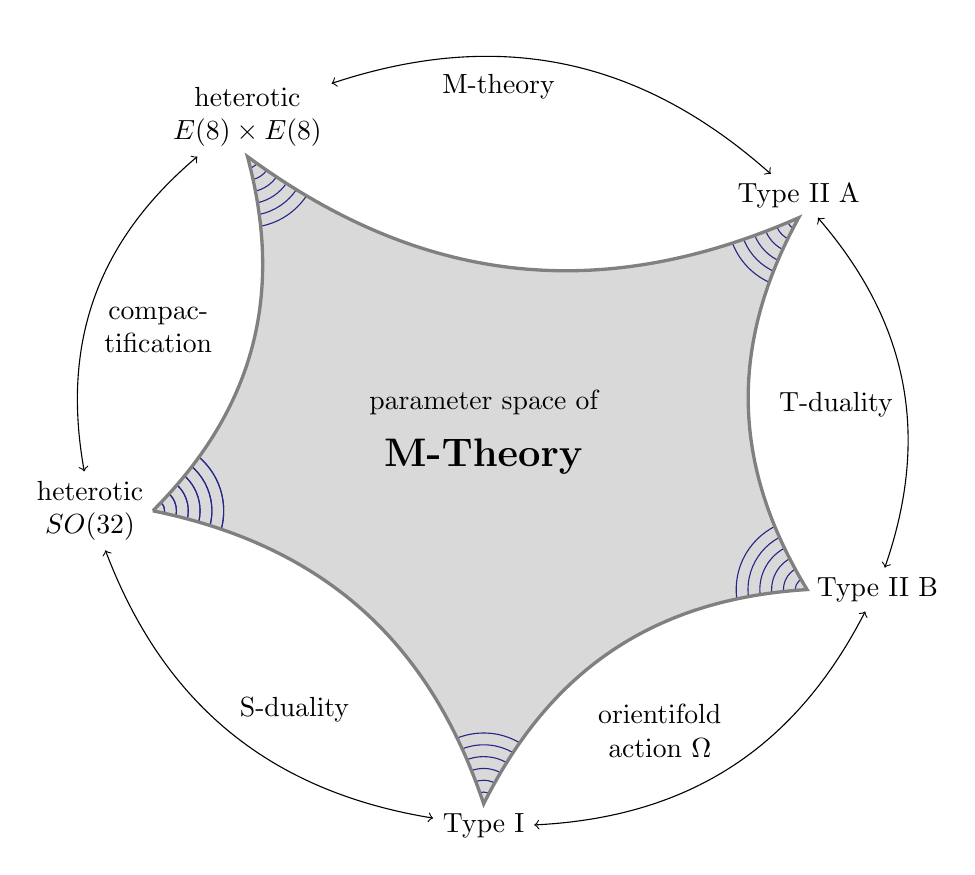
\begin{tikzpicture}

  \node (so32) [align=center] at (-5,-1) {heterotic\\$SO(32)$};
  \node (e8e8) [align=center] at (-3,4) {heterotic\\$E(8) \times E(8)$};
  \node (tiia) [align=center] at (4,3) {Type II A};
  \node (tiib) [align=center] at (5,-2) {Type II B};
  \node (ti) [align=center] at (0,-5) {Type I};

  \draw[bend left,<->] (so32) to node [below right,align=center] {compac-\\tification} (e8e8);
  \draw[bend left,<->] (e8e8) to node [below left] {M-theory} (tiia);
  \draw[bend left,<->] (tiia) to node [below left] {T-duality} (tiib);
  \draw[bend left,<->] (tiib) to node [above left,align=center] {orientifold\\action $\Omega$} (ti);
  \draw[bend left,<->] (ti) to node [above right] {S-duality} (so32);

  \begin{scope}
    \clip[bend right]
    (so32.east)
    to (e8e8.south)
    to (tiia.south)
    to (tiib.west)
    to (ti.north)
    to (so32.east);
    \foreach \c in {so32.east,e8e8.south,tiia.south,tiib.west,ti.north,so32.east}{%
        \foreach \r in {1,...,6}{%
            \draw[DarkBlue] (\c) circle (\r*0.15cm);
          }
      }
  \end{scope}

  \draw[bend right,very thick,gray,fill,fill opacity=0.3] (so32.east) to (e8e8.south) to (tiia.south) to (tiib.west) to (ti.north) to (so32.east);

  \node (mth) [align=center] at (0,0) {parameter space of\\[2ex]{\Large \textbf{M-Theory}}};

\end{tikzpicture}
\end{center}

\newpage
\tableofcontents
\newpage

\section{The Wave Function}

\subsection{The Schr\"{o}dinger Equation} \mbox{}\\

Imagine a particle of mass $m$, constrained to move along the $x$ axis, subject
to move to some specified force $F(x,t)$. The program of \textit{classical
mechanics} is to determine the position of the particle at any given time
$x(t)$. Once we know that, we can figure out the velocity $(v
= \frac{dx}{dt})$, the momentum $p = mv$, the kinetic energy $(T = \frac{1}{2}mv^2)$,
or any other dynamical variable of interest. To determine $x(t)$, we apply
Newton's Second Law: $F = ma$, or more specifically, $F = -\frac{\partial
V}{\partial x}$, the derivative of a potential energy function, where
$m\frac{\partial^2 x}{\partial t^2} = - \frac{\partial V}{\partial x}$. This
together, with initial conditions, determines $x(t)$. \\\\
Quantum mechanics approaches this same problem a bit differently. In this case
what we're looking for is the particles \textbf{wave function}, $\Phi(x,t)$,
and we get it by solving the \textbf{Schr\"{o}dinger Equation:} 
\\
\begin{tcolorbox}[colback = red!5!white, colframe = red!50!black, title
  = Schr\"{o}dinger Equation]

  \[
  i\hbar\frac{\partial \Psi}{\partial t} = - \frac{\hbar^2}{2m}\frac{\partial^2
  \Phi}{\partial x^2} + V\Phi
  \] 

\end{tcolorbox} \mbox{}\\


Here $i$ is the square root of $-1$, and $\hbar$ is Planck's constant - or
rather, his \textit{original} constant $(h)$ divided by  $2\pi$: 

\[
  \hbar = \frac{h}{2\pi} = 1.054573 \times 10^{-34} J s. 
\] \\

The Schro\"{o}dinger equation plays a role logically analogous to Newton's
second law. \\

\subsection{The Statistical Interpretation} \mbox{}\\


But what exactly \textit{is} this wave function, and what does it do for you
once you've \textit{got} it? After all a particle by nature is a point, whereas
the wave function (as its name suggests) is spread out in space (a function of
$x$, for any given  $t$). 

\begin{figure}[htb!]
  \centering
  \includegraphics[width = 10cm]{screenshot 12.png}
    \caption{a "particle" constrained to move in one dimension under the
    influence of a specified force}
\end{figure}

\begin{figure}[htb!]
  \centering
  \includegraphics[width = 10cm]{screenshot 13.png}
    \caption{a typical wave function. the shaded area represents the
    probability of finding the particle between $a$ and $b$. the particle would
  be relatively likely to be found near  $A$, and unlikely to be found near
$B$.}
\end{figure} 



How can such an object represent the state of a \textit{particle}? The answer
is provided by Born's \textbf{statistical interpretation}, which says that
$|\Psi(x,t)|^2$ gives the \textit{probability} of finding the particle at point
$x$, at time $t$ - or, more precisely, 
\\

\begin{tcolorbox}[colback = blue!5!white, colframe = blue!50!black, title
  = Born's Statistical Interpretation]
\[  
\int_{a}^{b} |\Psi(x,t)|^2\,dx = \{ \text{probability of finding particle
between $a$ and $b$, at time $t$ }\} 
\]
\end{tcolorbox} \mbox{}\\

Probability is the \textit{area} under the graph of $|\Psi|^2$. For the wave
function in the figure above, you would be quite likely to find the particle in
the vicinity of point A, where $|\Psi|^2$ is large, and relatively unlikely to
find it near point $B$. \\ \\ 

The statistical interpretation introduces a kind of \textbf{indeterminacy} into
quantum mechanics, for even if you know everything, the theory has to tell you
about the particle, still you can't predict with certainty the outcome of
a simple experiment to predict its position - all quantum mechanics has to
offer is \textit{statistical} information about \textit{possible} results. It
is natural to wonder whether this indeterminacy is a fact of nature, or
a defect in the theory. \\\\

Suppose I \textit{do} measure the position of the particle, and I find it to be
a point $C$. \mbox{}\\ 

\textbf{\textit{Question}}\\\\
Where was the particle just  \textit{before} I made the measurement? \\\\

\textbf{\textit{Solution}}\\\\
There are three plausible answers \mbox{}\\

\begin{tcolorbox}	
  
  1. The \textbf{realist} position: The \textit{particle was at} $C$. This
     certainly seems reasonable, and it is the response Einstein advocated.
     However, if this is true, quantum mechanics is an \textit{incomplete}
     theory, since the particle \textit{really was} at $C$, and yet quantum
     mechanics was unable to tell us so. 

\end{tcolorbox} \mbox{}\\

\begin{tcolorbox}	
  
  2. The \textbf{orthodox} position: The \textit{particle wasn't really
anywhere}. It was the act of measurement that forced it to "take a stand"
(though how and why it chose the point $C$ we dare not ask). This view is
associated with Bohr and his followers. Among physicists it is the most widely
accepted position. However, if it is correct, a century worth of debate about
the act of measurement has done preciously little to illuminate. 

\end{tcolorbox}	\mbox{}\\

\begin{tcolorbox}	
  
  The \textbf{agnostic} position: \textit{Refuse to answer}. This is not as
  silly as it sounds - what sense can there be in making assertions about the
  status of a particle \textit{before} a measurement. For decades this was the
  "fall-back" position of most physicists: they'd try to sell you the orthodox
  answer, but if you were persistent they'd retreat to the agnostic response,
  and terminate the conversation.

\end{tcolorbox}	\mbox{}\\




\end{document}  

